\section{Observational Geometry: Reconstructing Response from Experiment}
\label{sec:observational}
The preceding sections developed the intrinsic geometry of
nonequilibrium response. Beginning with quasistatic evolution on
the Liouvillian control manifold, we showed that open quantum
systems possess a natural geometric structure defined by a work
one-form, its associated curvature, and a local response tensor
whose symmetric and antisymmetric components describe reciprocal
and nonreciprocal response. These objects are intrinsic
properties of the stationary-state manifold. Like the metric and
curvature tensors of differential geometry, they exist
independently of any particular experimental realization.
Physical measurements, however, do not access these intrinsic
geometric quantities directly. Spectroscopic experiments probe
transition amplitudes, optical coherences, and time-dependent
polarization, whereas the response metric and curvature are
properties of the parameter-dependent Liouvillian governing the
underlying dynamics. The central challenge is therefore one of
geometric reconstruction: how may the intrinsic geometry of the
response manifold be inferred from experimentally observable
signals?

The answer developed in our recent work is to reinterpret
nonlinear spectroscopy as a problem in geometric transport.
Conventional response theory expands the density operator in
powers of the external optical field while holding the
Liouvillian fixed. This approach successfully describes the
generation of nonlinear optical signals but implicitly assumes
that the generator of the dynamics is known exactly. In practice,
however, microscopic models are necessarily approximate.
Important physical processes---including environmental
fluctuations, correlated dissipation, spin-orbit coupling,
vibronic interactions, and collective many-body effects---are
often neglected in an initial description and subsequently
introduced through increasingly sophisticated Hamiltonians or
system--bath models.

From the perspective of response geometry, these additional
physical interactions should not be viewed merely as corrections
to the calculated spectrum. Rather, they modify the generator of
the dynamics itself and therefore alter the geometry of the
underlying response manifold. Improving the microscopic model is
thus equivalent to refining the geometric description of the
system. The experimentally observed spectrum changes because the
local response geometry has changed.

This observation suggests a natural extension of conventional
perturbation theory. Instead of expanding only the interaction
with the optical field, we regard the Liouvillian itself as a
parameter-dependent object,
\begin{align}
\mathcal L
=
\mathcal L(\lambda),
\end{align}
where the control coordinates
$\lambda=(\lambda^1,\lambda^2,\ldots)$
may represent external fields, temperatures, system--bath
couplings, or other experimentally tunable parameters. Motion
through this control manifold induces corresponding changes in
the generator of the dynamics,
\begin{align}
\mathcal L(\lambda+\delta\lambda)
=
\mathcal L(\lambda)
+
\delta\lambda^\mu
\partial_\mu\mathcal L
+
\frac12
\delta\lambda^\mu
\delta\lambda^\nu
\partial_\mu\partial_\nu\mathcal L
+\cdots.
\end{align}
The problem therefore becomes one of transporting observables
through a continuously varying family of Liouvillian generators.
This shift in perspective represents the principal conceptual
advance of the observational framework. Conventional nonlinear
spectroscopy reconstructs dynamical response by perturbatively
expanding the interaction with the radiation field. Here the
perturbation parameter is instead the motion of the Liouvillian
through the response manifold itself. The resulting Duhamel
expansion naturally defines transport operators that connect
observable spectroscopic signals with the intrinsic metric and
curvature developed in the preceding sections. In this way,
response geometry becomes experimentally accessible, completing
the progression from intrinsic geometry to observable geometry.


\begin{tcolorbox}[
colback=gray!5,
colframe=black,
title=\textbf{Principle of Geometric Refinement},
fonttitle=\bfseries,
breakable]
\textbf{Microscopic model refinement is equivalent to geometric refinement.}
Traditional spectroscopy systematically improves microscopic
Hamiltonians or system--bath models until the calculated spectra
reproduce experiment. Within the framework developed here, this
process admits a complementary geometric interpretation. Each
additional physical interaction modifies the Liouvillian
generator and therefore deforms the local response geometry.
The experimentally observed spectrum changes because the
underlying response manifold has been refined.
The Duhamel expansion provides the differential calculus
governing this geometric refinement. Rather than simply adding
perturbative corrections to the dynamics, it describes how the
response metric, curvature, and observable transport evolve as
the microscopic description becomes progressively more complete.
From this perspective, nonlinear spectroscopy is no longer
viewed primarily as a method for determining Hamiltonian
parameters, but as a means of reconstructing and refining the
geometry of physical response.
\end{tcolorbox}

\subsection{Differential Geometry of Liouville Space}
\label{subsec:liouville_geometry}
The preceding sections established the intrinsic geometry of
thermodynamic response. Metrics and curvature characterize the
response of stationary states to variations of external control
parameters and determine the local and global structure of
nonequilibrium thermodynamics. Spectroscopic measurements,
however, do not probe stationary states directly. They interrogate
the dynamical evolution of optical coherences and populations,
requiring a geometric description of transport on the manifold of
Liouvillian generators rather than on the manifold of stationary
states alone.

This distinction is fundamental. The response curvature
$F_{\mu\nu}$ introduced earlier governs quasistatic work and
nonreciprocal thermodynamic response. Spectroscopy instead probes
how dynamical pathways evolve as the generator of the dynamics is
varied. The relevant geometric objects are therefore connections
and curvature defined on the Liouvillian manifold itself.

\subsubsection{Transport of Liouvillian Eigenoperators}
Consider a parameter-dependent Liouvillian
\begin{align}
\mathcal L=\mathcal L(\lambda),
\end{align}
where the control coordinates
$\lambda^\mu=(\lambda^1,\lambda^2,\ldots)$
may represent thermodynamic variables, external fields,
pulse-sequence parameters, system--bath couplings, or other
experimentally tunable quantities. The corresponding
Liouvillian eigenproblem is
\begin{align}
\mathcal L(\lambda)\Phi_n(\lambda)
=
\Lambda_n(\lambda)\Phi_n(\lambda),
\end{align}
together with the biorthogonal left eigenoperators
\begin{align}
\widetilde\Phi_m^\dagger(\lambda)
\mathcal L(\lambda)
=
\Lambda_m(\lambda)
\widetilde\Phi_m^\dagger(\lambda),
\end{align}
normalized according to
\begin{align}
\langle\!\langle
\widetilde\Phi_m
|
\Phi_n
\rangle\!\rangle
=
\delta_{mn}.
\end{align}
As the control parameters vary, both the eigenvalues and the
eigenoperators evolve. These two forms of variation have
fundamentally different physical consequences.
Changes in the eigenvalues modify oscillation frequencies,
relaxation rates, and dephasing times, but do not alter the
underlying organization of spectroscopic pathways. By contrast,
changes in the eigenoperators modify the Liouville-space basis
itself, transporting populations and coherences between
pathways. Geometry therefore resides not in the evolution of the
Liouvillian spectrum, but in the evolution of its eigenoperators.

A simple example is provided by pure dephasing. The decoherence
rate may depend strongly upon temperature while the
eigenoperators remain fixed. In that case the spectrum changes,
yet no geometric pathway transport occurs. Nontrivial geometric
response emerges only when the eigenoperators themselves evolve
with the control parameters.

\begin{tcolorbox}[
colback=gray!5,
colframe=black,
title=\textbf{Principle of Pathway Geometry},
fonttitle=\bfseries]
Geometric transport is governed by the evolution of
Liouvillian eigenoperators, not by the evolution of
Liouvillian eigenvalues. Eigenvalues determine rates;
eigenoperators determine geometry.
\end{tcolorbox}

\subsubsection{Liouvillian Connections}
Comparing pathway bases defined at neighboring points of the
control manifold requires a rule for parallel transport. The
appropriate object is the Liouvillian connection,
\begin{align}
\Gamma_\mu
=
\partial_\mu\mathcal L,
\end{align}
which measures the local deformation of the generator under an
infinitesimal displacement in parameter space.
Expressed in the local Liouvillian eigenbasis,
\begin{align}
(\Gamma_\mu)_{mn}
=
\langle\!\langle
\widetilde\Phi_m
|
\Gamma_\mu
|
\Phi_n
\rangle\!\rangle,
\end{align}
the diagonal elements describe the response of individual
pathways, while the off-diagonal elements couple distinct
pathways and generate transport throughout the Liouville-space
network.

The Liouvillian connection plays a role analogous to the Berry
connection for adiabatic quantum evolution. The difference is
that the transported objects are not wavefunctions but
Liouvillian eigenoperators and the spectroscopic pathways they
define. Consequently, Liouvillian geometry naturally incorporates
dissipation, decoherence, and environmental interactions, all of
which lie outside conventional Berry theory.
\subsubsection{Curvature and Pathway Transport}
Transport generated by different physical mechanisms generally
does not commute. Coherent evolution, dissipation,
system--bath interactions, and optical driving define competing
transport directions in Liouville space,
\begin{align}
\mathcal L
=
\mathcal L_H
+
\mathcal L_D
+
\mathcal L_{\rm int}
+\cdots,
\end{align}
with
\begin{align}
[
\mathcal L_\alpha,
\mathcal L_\beta
]
\neq0.
\end{align}
The incompatibility of these transport directions is quantified
by the Liouvillian curvature,
\begin{align}
\mathcal K_{\mu\nu}
=
\partial_\mu\Gamma_\nu
-
\partial_\nu\Gamma_\mu
+
[
\Gamma_\mu,\Gamma_\nu
].
\end{align}
This curvature measures the failure of successive transport
operations to commute and therefore quantifies the intrinsic
geometry of pathway transport.

Transport around a closed loop generates the Liouvillian
holonomy,
\begin{align}
\mathcal U_C
=
\mathcal P
\exp
\left[
\oint_C
\Gamma_\mu
d\lambda^\mu
\right],
\end{align}
which represents the cumulative geometric transformation of the
pathway basis.

\subsubsection{Observable Bundles and Observational Holonomy}
The full Liouville-space transport is not directly accessible to
experiment. Spectroscopy measures
\begin{align}
S(t)
=
{\rm Tr}
[
O\rho(t)
],
\end{align}
where the observable $O$ projects the evolving density operator
onto a particular measurement channel. Every spectroscopic
experiment therefore defines an induced observable bundle obtained
by projecting the intrinsic Liouville bundle onto the subspace
selected by the preparation and detection operators.
The experimentally observed transport is consequently not the
full Liouvillian holonomy but its projection onto this observable
bundle. We refer to this projected quantity as the
\emph{observational holonomy}. Different observables probe
different projections of the same underlying Liouvillian
transport and therefore need not reveal identical geometric
structure
.
Observation is therefore itself a geometric operation. The
measured spectrum resides not on the intrinsic Liouvillian
manifold but on an observable manifold induced by the
measurement process. Reconstructing response geometry from
spectroscopy is therefore simultaneously a problem of dynamical
transport and observable projection.

\subsubsection{Geometric Refinement}
The differential geometry developed above provides the intrinsic
description of Liouville-space transport. The remaining question
is computational: given an approximate Liouvillian, how does one
systematically refine its geometry until the predicted
observational holonomy agrees with experiment?

Within the present framework, improving a microscopic model is
equivalent to refining its response geometry. Each additional
physical interaction modifies the Liouvillian connection and
curvature, thereby deforming the local geometry of pathway
transport. The Duhamel expansion introduced in the following
section provides the differential calculus governing this process
of geometric refinement.


%at end
\begin{tcolorbox}[
colback=gray!5,
colframe=black,
title=\textbf{Principle of Observational Holonomy},
fonttitle=\bfseries,
breakable]
The Liouvillian connection defines the transport of dynamical
pathways on the manifold of generators. Spectroscopic
measurements, however, do not observe this transport directly.
Instead, they measure only its projection onto the observable
subspace selected by the preparation and detection operators.
Consequently, the experimentally reconstructed holonomy is not
the full Liouville-space holonomy, but the holonomy induced on
the observable subspace. Observation is therefore a geometric
projection, and different spectroscopic protocols reconstruct
different projections of the same underlying response geometry.
The basis-misalignment angle $\theta$ is the local coordinate
parameterizing this observable projection. Reconstructing
$\theta$ from nonlinear spectra is therefore equivalent to
reconstructing the local observational geometry.
\end{tcolorbox}




\subsection{The Canonical Two-Level Coordinate Chart}
\label{subsec:canonical2LS}
The differential geometry developed in the preceding section is
completely general and applies to arbitrary open quantum systems.
To expose its essential structure, however, it is useful to
introduce the simplest nontrivial realization of observational
geometry. Rather than viewing the two-level system as a minimal
model, we regard it as the canonical local coordinate chart on
the manifold of Liouvillian geometries.

The privileged role of the two-level system in quantum mechanics
extends naturally to observational geometry. Just as the tangent
plane provides a local coordinate chart for a differentiable
manifold, the canonical two-level system provides the simplest
local coordinate chart for the manifold of Liouvillian
geometries. Although realistic open quantum systems generally
possess high-dimensional response manifolds with many interacting
pathways, their local geometric structure is frequently governed
by the effective coupling of a pair of pathways. The single
observational coordinate $\theta$ therefore captures the leading
local deformation of the observable bundle in precisely the same
way that local coordinates describe the neighborhood of a point
on a manifold. Higher-dimensional systems require additional
geometric coordinates, but the underlying notions of Liouvillian
connection, curvature, pathway transport, and observational
holonomy remain unchanged. The canonical two-level system should
therefore be viewed not as a special physical model, but as the
\textit{universal local chart from which the differential geometry of
observational response is constructed.}

The same canonical two-level system has appeared throughout the
development of the present framework. In our earlier work on
stationary-state response, it provided the simplest realization
of response geometry, illustrating how the misalignment between
the Hamiltonian and pointer bases generates a symmetric response
metric together with an antisymmetric curvature two-form. Here,
the physical model remains unchanged, but the question is
different. Rather than asking how this geometry determines
quasistatic work performed around a closed control cycle, we ask
how it manifests itself in nonlinear optical measurements.

Observation therefore introduces an additional geometric layer:
the transport of observable pathways through Liouville space.
The canonical model consists of a two-level Hamiltonian,
\begin{align}
H=\frac{\Delta}{2}\sigma_z,
\end{align}
whose eigenstates define the observational basis used by the
spectroscopic experiment. In the absence of environmental
coupling, these states generate the familiar independent
Liouville-space pathways that underlie the conventional
decomposition of the nonlinear response.
The environment, however, selects its own preferred pointer
basis, related to the observational basis through the unitary
transformation
\begin{align}
|p_n\rangle
=
U(\theta)
|e_n\rangle,
\end{align}
where $\theta$ is the local coordinate of the canonical
observable chart. Physically, $\theta$ is realized as the
misalignment between the observational basis defined by the
experiment and the pointer basis selected by the environment.
Geometrically, however, it is more fundamental: it parameterizes
the local deformation of the observable bundle induced by
environmental interactions.

When $\theta=0$, the observational and pointer bases coincide.
The dissipative dynamics reduce to pure dephasing in the
observational basis, Liouville-space pathways remain independent,
and no observational transport is generated. As $\theta$
increases, environmental monitoring mixes populations and
coherences, activating transport between pathways and generating
the observational geometry described in the previous section.
Recovering $\theta$ from nonlinear spectroscopic measurements is
therefore equivalent to reconstructing the leading local
deformation of the observable bundle.
The two-level system is therefore not important because it is
simple, but because it exposes the local differential geometry in
its most transparent form. More complex systems require
additional coordinates and a corresponding atlas of overlapping
coordinate charts, yet the underlying geometric construction
remains unchanged. The canonical two-level chart thus plays the
same role in observational geometry that the tangent plane plays
in differential geometry: it provides the universal local model
from which the global geometry is assembled.




\subsection{Liouville Propagator Expansion and the Transport Matrix}
\label{subsec:duhamel_transport}
The canonical two-level chart identifies the local observational
coordinate \(\theta\), but it does not by itself determine how
spectroscopic pathways are transported. To compute that transport
we require a perturbative expansion of the Liouville propagator.
This is the point at which the Duhamel expansion enters: not as
the starting point of the theory, but as the calculational
machinery for refining the local Liouvillian geometry.

Let the Liouvillian depend smoothly on a set of local deformation
coordinates \(\lambda^\mu\). Near a reference Liouvillian
\(\mathcal L_0=\mathcal L(\lambda=0)\), we write
\begin{align}
\mathcal L(\lambda)
=
\mathcal L_0
+
\lambda^\mu \mathcal X_\mu
+
\frac12
\lambda^\mu\lambda^\nu
\mathcal Y_{\mu\nu}
+
O(\lambda^3),
\label{eq:L_local_expansion}
\end{align}
where
\begin{align}
\mathcal X_\mu
&=
\left.
\partial_\mu\mathcal L
\right|_{\lambda=0},
&
\mathcal Y_{\mu\nu}
&=
\left.
\partial_\mu\partial_\nu\mathcal L
\right|_{\lambda=0}.
\end{align}
The operators \(\mathcal X_\mu\) are tangent vectors on the
manifold of Liouvillian geometries. They identify the leading
directions in which the generator is deformed away from the
reference dynamics. The tensors \(\mathcal Y_{\mu\nu}\) describe
the local nonlinear deformation of this manifold. In the canonical
two-level chart the coordinate manifold is one-dimensional and
\(\lambda^\mu\rightarrow\theta\), so that
\begin{align}
\mathcal L(\theta)
=
\mathcal L_0
+
\theta\mathcal X
+
\frac{\theta^2}{2}\mathcal Y
+
O(\theta^3).
\label{eq:L_theta_expansion_review}
\end{align}
The propagator over a waiting interval \(\tau\) is
\begin{align}
U(\tau;\lambda)
=
\exp\left[
\mathcal L(\lambda)\tau
\right].
\end{align}
Because \(\mathcal L_0\) and the deformation operators generally
do not commute, the exponential cannot be expanded as an ordinary
scalar Taylor series. The appropriate expansion is the Duhamel
series, which expresses the perturbed propagator as insertions of
the deformation operators into the reference evolution. To second
order,
\begin{align}
U(\tau;\lambda)
=
U_0(\tau)
+
\lambda^\mu U^{(1)}_\mu(\tau)
+
\frac12
\lambda^\mu\lambda^\nu
U^{(2)}_{\mu\nu}(\tau)
+
O(\lambda^3),
\label{eq:U_duhamel_review}
\end{align}
with
\begin{align}
U_0(\tau)
=
e^{\mathcal L_0\tau},
\end{align}
and
\begin{align}
U^{(1)}_\mu(\tau)
=
\int_0^\tau ds\,
e^{\mathcal L_0(\tau-s)}
\mathcal X_\mu
e^{\mathcal L_0 s}.
\label{eq:U1_duhamel_review}
\end{align}
The first-order term describes a single deformation event inserted
at time \(s\), propagated before and after by the reference
Liouvillian.

The second-order contribution contains two distinct pieces:
\begin{align}
U^{(2)}_{\mu\nu}(\tau)
&=
\int_0^\tau ds\,
e^{\mathcal L_0(\tau-s)}
\mathcal Y_{\mu\nu}
e^{\mathcal L_0 s}
\nonumber\\
&\quad
+
2
\int_0^\tau ds
\int_0^s ds'\,
e^{\mathcal L_0(\tau-s)}
\mathcal X_\mu
e^{\mathcal L_0(s-s')}
\mathcal X_\nu
e^{\mathcal L_0s'} .
\label{eq:U2_duhamel_review}
\end{align}
The first term is a single insertion of the second-order
deformation \(\mathcal Y_{\mu\nu}\). The second is a double
insertion of the first-order tangent operators
\(\mathcal X_\mu\) and \(\mathcal X_\nu\), separated by free
evolution under \(\mathcal L_0\). This term is the explicit
Liouville-space expression of pathway transport generated by
successive noncommuting deformations.

To connect this propagator expansion to spectroscopy, let
\(\{S_a^{(0)}\}\) denote the conventional zeroth-order pathway
decomposition of the nonlinear signal,
\begin{align}
S^{(0)}
=
\sum_a S_a^{(0)} .
\end{align}
In the reference geometry each pathway evolves independently. A
deformation of the Liouvillian transports amplitude among these
pathways, so that the observed pathway amplitudes may be written
as
\begin{align}
S_a(\lambda)
=
\sum_b
T_{ab}(\lambda)
S_b^{(0)} .
\label{eq:pathway_transport_review}
\end{align}
The matrix \(T_{ab}\) is the observable transport matrix. It is
the representation of Liouville-space transport on the
experimentally accessible pathway basis. Its diagonal elements
renormalize individual pathway weights, while its off-diagonal
elements quantify transfer of amplitude between pathways.

Projecting the Duhamel-expanded propagator onto the zeroth-order
pathway basis gives
\begin{align}
T_{ab}(\lambda)
=
\delta_{ab}
+
\lambda^\mu T^{(1)}_{ab,\mu}
+
\frac12
\lambda^\mu\lambda^\nu
T^{(2)}_{ab,\mu\nu}
+
O(\lambda^3).
\label{eq:T_expansion_review}
\end{align}
The coefficients \(T^{(1)}_{ab,\mu}\) are obtained by inserting
\(U^{(1)}_\mu\) into the corresponding Liouville pathway
expression, while \(T^{(2)}_{ab,\mu\nu}\) are obtained from
\(U^{(2)}_{\mu\nu}\). Thus the transport matrix is not an
independent phenomenological fitting object. It is the projected
representation of the local Liouvillian deformation on the
observable bundle.

For the canonical two-level chart this reduces to
\begin{align}
T_{ab}(\theta)
=
\delta_{ab}
+
\theta T^{(1)}_{ab}
+
\frac{\theta^2}{2}
T^{(2)}_{ab}
+
O(\theta^3).
\label{eq:T_theta_review}
\end{align}
The experimentally reconstructed parameter \(\theta\) is therefore
not merely a basis-misalignment angle. It is the local coordinate
that determines how the observable pathway basis is transported
away from the reference geometry. Reconstructing \(\theta\) from
nonlinear spectra is equivalent to reconstructing the leading
deformation of the observable bundle.

It is useful to distinguish the Taylor coefficients
\(\mathcal Y_{\mu\nu}\) from the Liouvillian curvature
\(\mathcal K_{\mu\nu}\). The former describe local nonlinear
changes of the generator in a chosen coordinate chart. The latter
is constructed from the Liouvillian connection and measures the
failure of transport operations to commute:
\begin{align}
\mathcal K_{\mu\nu}
=
\partial_\mu\Gamma_\nu
-
\partial_\nu\Gamma_\mu
+
[\Gamma_\mu,\Gamma_\nu].
\end{align}
Both arise from the same underlying Liouvillian geometry, but
they encode different information. The tensors
\(\mathcal Y_{\mu\nu}\) describe the local shape of the generator
manifold, while \(\mathcal K_{\mu\nu}\) describes the curvature
of transport on that manifold.

Equations~\eqref{eq:U_duhamel_review}--\eqref{eq:T_theta_review}
give the operational form of geometric refinement. Beginning from
a reference Liouvillian, additional physical interactions deform
the generator, transport amplitude among observable pathways, and
alter the measured nonlinear spectrum. The Duhamel expansion is
therefore not simply a perturbative correction to the signal. It
is the differential calculus by which the local response geometry
is refined and projected into experimentally measurable form.

\subsection{Liouville Pathways as an Observable Basis}
\label{subsec:pathway_basis}
Nonlinear optical spectroscopy is traditionally formulated as a
sum over Liouville-space pathways, each represented by a
double-sided Feynman diagram specifying a particular sequence of
light--matter interactions and free evolution. The third-order
polarization may be written schematically as
%
\begin{align}
P^{(3)}(t)
=
\sum_a
S_a(t),
\label{eq:P3sum}
\end{align}
%
where the index $a$ labels every Liouville pathway contributing
to the measured signal. Depending upon the system under
consideration, these include rephasing and non-rephasing
contributions arising from ground-state bleach (GSB), stimulated
emission (SE), excited-state absorption (ESA), double-quantum
coherences, and higher-order processes. The experimentally
observed spectrum is obtained only after coherent summation over
all contributing pathways.
Conventionally, the individual Liouville pathways are regarded as
diagrammatic bookkeeping devices that organize the perturbation
expansion of the nonlinear response. Within the present
framework, however, they admit a deeper geometric
interpretation. The collection of pathway amplitudes
%
\begin{align}
\mathbf{S}
=
\left(
S_1,
S_2,
\ldots,
S_N
\right)^T
\end{align}
%
forms a natural basis for the observable bundle associated with
the chosen experiment. The individual Liouville pathways are
therefore not merely contributions to the spectrum, but basis
vectors spanning the space of experimentally accessible
responses.

The geometric role of the Liouvillian is to transport this basis
through the manifold of response geometries. As the Liouvillian
is deformed by changes in the system Hamiltonian, environmental
couplings, external fields, or thermodynamic conditions, pathway
amplitudes are redistributed throughout the observable basis.
The response is therefore no longer described by independent
Liouville pathways, but by a transported basis,
%
\begin{align}
S_a
=
\sum_b
T_{ab}
S_b^{(0)},
\label{eq:Ttransport}
\end{align}
%
where $S_b^{(0)}$ denotes the reference pathway amplitudes and
$T_{ab}$ is the observable transport operator. The operator
itself is intrinsic to the Liouvillian geometry, while the matrix
elements shown above are its representation in the chosen
Liouville-pathway basis. The diagonal elements describe the
renormalization of individual pathway amplitudes, whereas the
off-diagonal elements quantify transport between distinct
Liouville pathways generated by the environment.

For the canonical two-level coordinate chart introduced in the
previous section, the observable basis is particularly compact.
The third-order response contains only the GSB and ESA
contributions, each possessing both rephasing and non-rephasing
sectors, so that the complete signal is obtained by summing over
all transported Liouville pathways. The resulting transport
operator is therefore of low dimension, making the underlying
geometry especially transparent. In realistic molecular and
condensed-phase systems, the observable bundle expands to include
many additional pathways, but the geometric construction remains
unchanged. The transport operator continues to describe the
evolution of the complete Liouville-pathway basis; only the
dimension of the observable bundle increases.

This interpretation establishes a direct correspondence between
the differential geometry developed in the preceding sections and
the familiar diagrammatic language of nonlinear spectroscopy.
Liouville pathways play the role of local basis vectors for the
observable bundle, the Liouvillian connection specifies their
infinitesimal transport, the curvature measures the
noncommutativity of successive transport operations, and the
observed nonlinear spectrum is the projection of the transported
basis onto the experimental detection channel. From this
perspective, nonlinear spectroscopy is naturally reinterpreted as
a measurement of the transport of an observable basis through the
manifold of Liouvillian geometries.


\section{Numerical Demonstration of Geometric Reconstruction}
\label{sec:numerics}
The preceding sections established the theoretical framework
underlying observational geometry. The remaining question is
whether the local geometric coordinates can, in practice, be
reconstructed from nonlinear spectroscopic data. We now
illustrate this reconstruction using the canonical two-level
coordinate chart developed above. Although deliberately simple,
this model contains all of the essential ingredients of the
geometric theory while permitting direct comparison between exact
Liouvillian propagation and the Duhamel transport expansion.

\begin{figure*}
\centering
\begin{minipage}{0.48\textwidth}
\centering
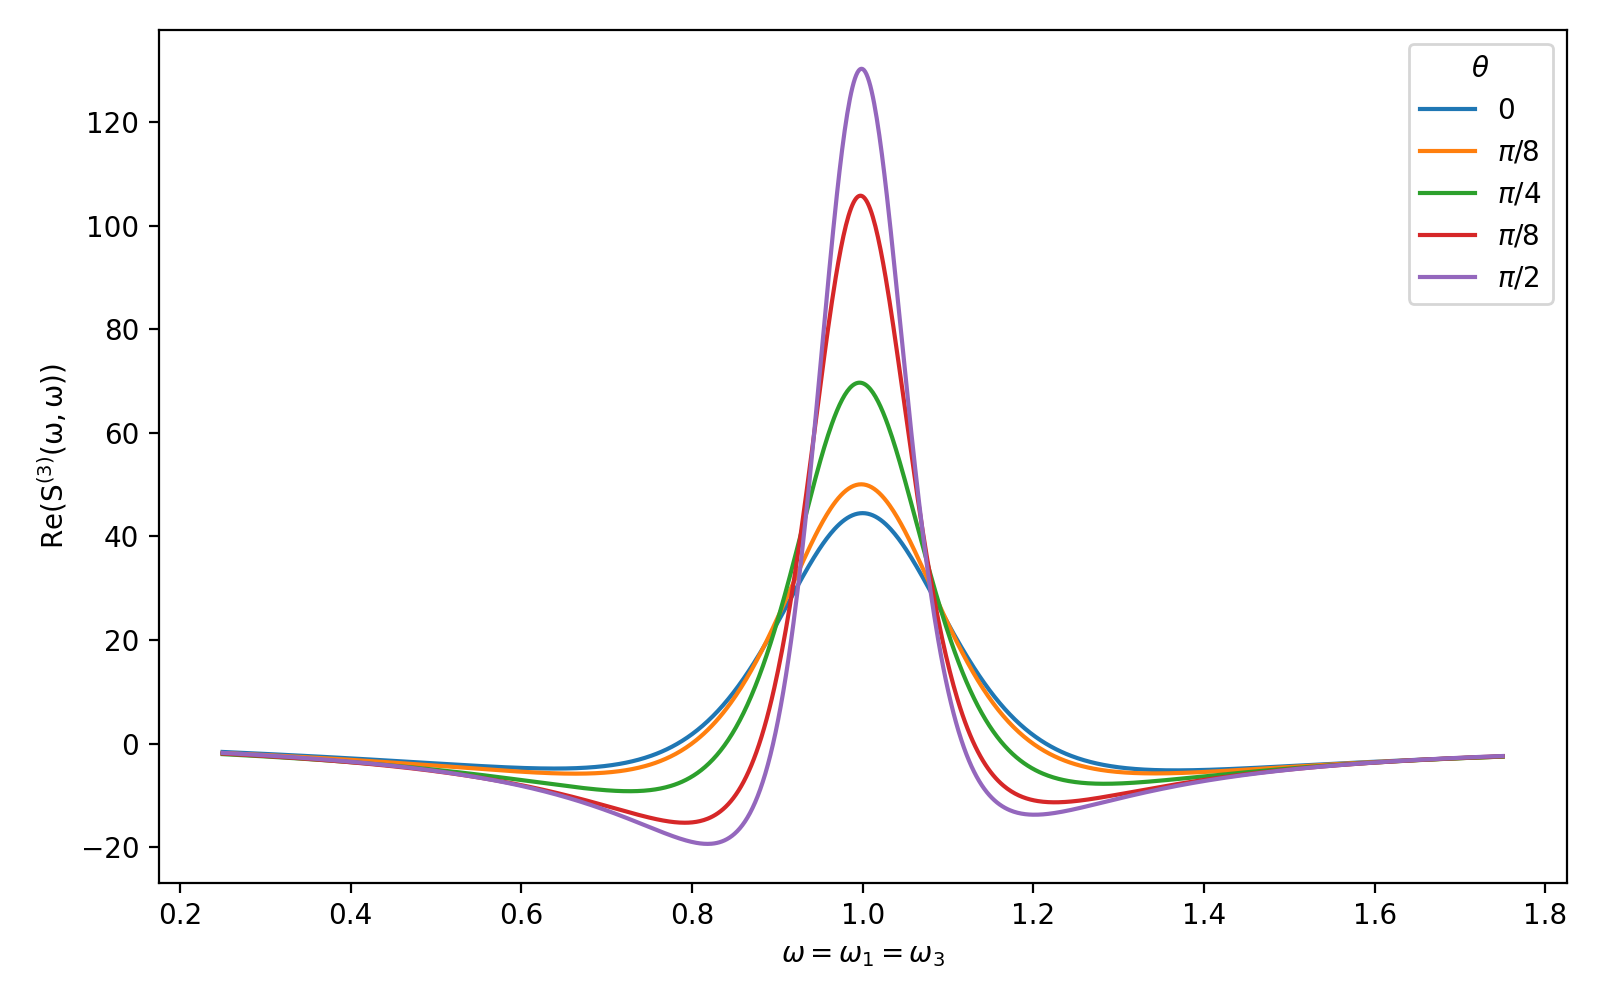
\includegraphics[width=\linewidth]{Figures/corrected_diag_theta_real_2.png}
\end{minipage}
\hfill
\begin{minipage}{0.48\textwidth}
\centering
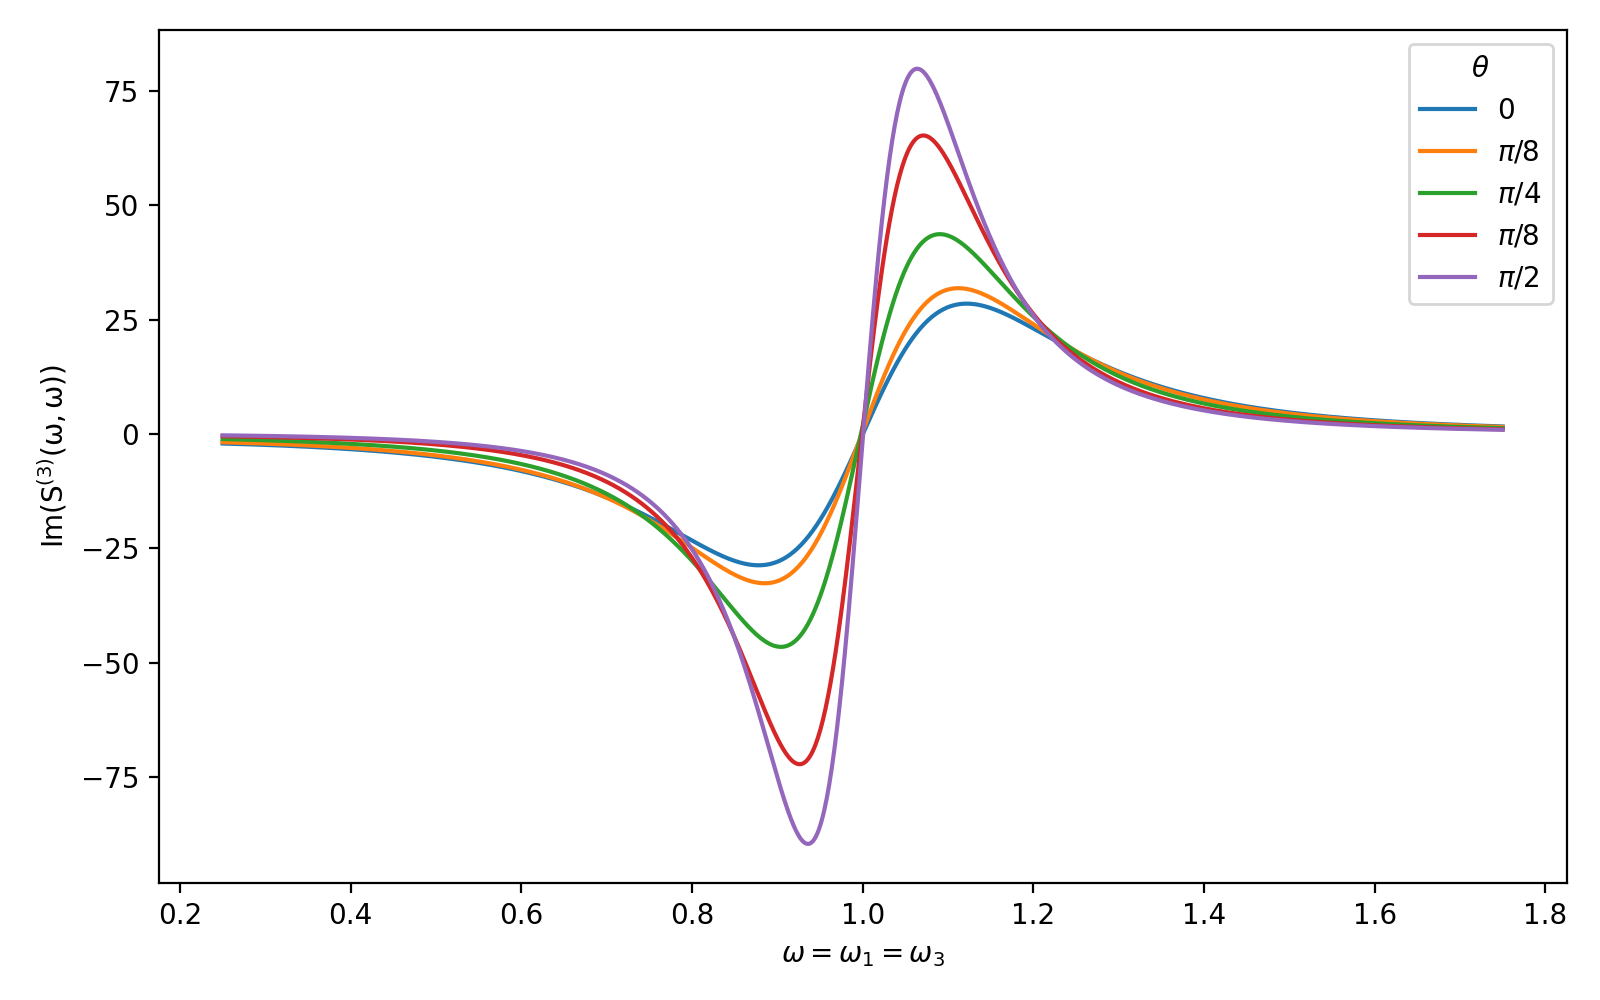
\includegraphics[width=\linewidth]{Figures/corrected_diag_theta_imag_2.png}
\end{minipage}
\caption{Real (left) and imaginary (right) components 
of the diagonal spectral response for increasing 
pointer-basis misalignment $\theta$. At $\theta = 0$, 
only dephasing contributions are present. For 
$\theta \neq 0$, basis misalignment mixes response 
pathways, producing continuous and structured 
deformations of the complex spectrum. These serve 
as benchmarks for the Duhamel reconstructions shown 
in Fig.~\ref{fig:TransportError}.}
\label{fig:DiagResponse}
\end{figure*}

\subsection{Spectroscopic Fingerprints of the Observable Bundle}
Figure~\ref{fig:DiagResponse} shows representative diagonal
spectral slices obtained from the full third-order response for
increasing values of the observational coordinate $\theta$. The
reported spectra include the complete third-order signal,
obtained by coherently summing all contributing Liouville
pathways, including both rephasing and non-rephasing sectors.
Within the canonical two-level chart these consist of the
ground-state bleach and excited-state absorption pathways
together with their corresponding rephasing and non-rephasing
contributions.

The Hamiltonian and optical transition operators are held fixed
throughout the calculation so that all observed spectral changes
originate solely from deformation of the Liouvillian geometry.
As the observational coordinate increases, transport between
Liouville pathways continuously redistributes both spectral
weight and phase, producing characteristic distortions in the
real and imaginary components of the nonlinear response.
The important observation is that these distortions are highly
structured and evolve continuously with $\theta$. The observable
coordinate therefore possesses a unique spectroscopic
fingerprint, establishing the forward mapping
\[
\theta
\longrightarrow
P^{(3)}(\omega_1,\omega_3),
\]
which forms the basis for geometric reconstruction.

\subsection{Accuracy of the Geometric Refinement}
The Duhamel expansion provides a systematic approximation to the
transport operator by successively refining the local
Liouvillian geometry. Figure~\ref{fig:TransportError} compares
the reconstruction error obtained from the zeroth-, first-, and
second-order transport expansions.

\begin{figure}
\centering
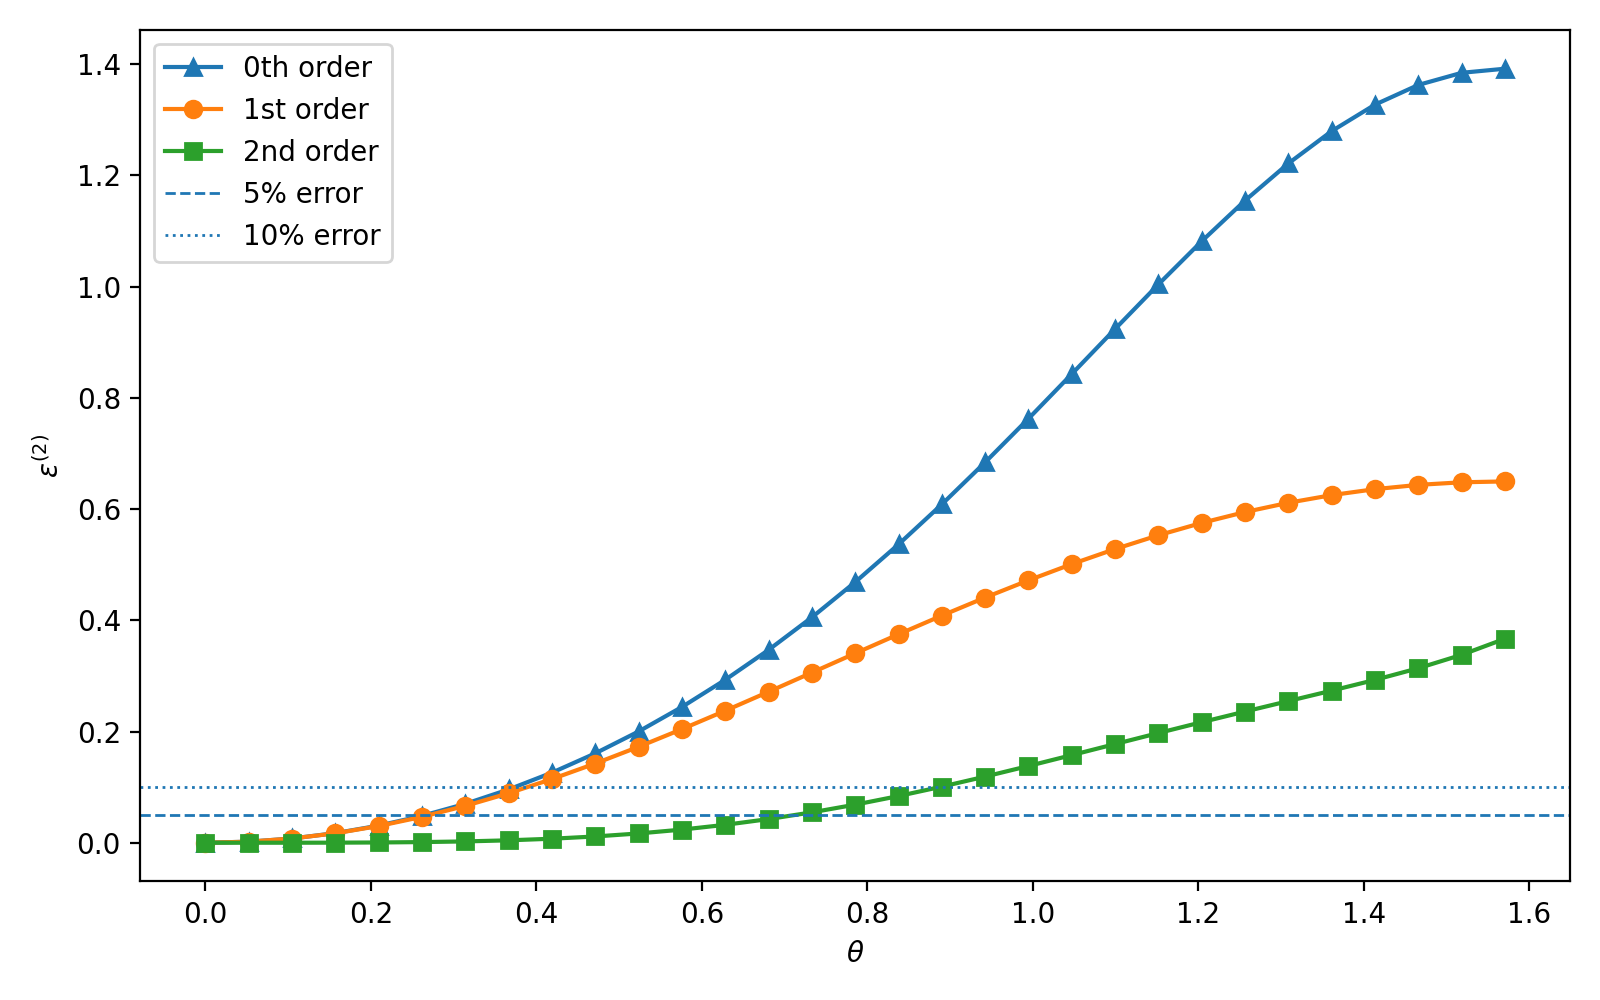
\includegraphics[width=0.75\linewidth]{Figures/duhamel_second_order_error_scaling_2.png}
\caption{Global reconstruction error $\epsilon^{(n)}$ 
for the first- and second-order Duhamel transport 
expansions as a function of pointer-basis misalignment 
$\theta$. The zeroth-order curve compares the 
$\theta = 0$ signal to the exact result at 
$\theta \neq 0$. The second-order approximation 
remains accurate throughout the full range of 
misalignment, including at $\theta = \pi/2$ where 
the observational and pointer bases are maximally 
misaligned.}
\label{fig:TransportError}
\end{figure}



Several features are noteworthy. First, the zeroth-order
approximation fails rapidly once the observational and pointer
bases become misaligned, illustrating that pathway transport is
an essential component of the nonlinear response. Second, the
first-order transport operator captures the dominant effects of
Liouville-space transport. Finally, inclusion of the second-order
terms reduces the reconstruction error by more than an order of
magnitude and remains quantitatively accurate over the entire
range of observational coordinates examined.

This behavior has a clear geometric interpretation. Although the
transport operator is constructed from a local expansion about
the reference geometry at $\theta=0$, the resulting coordinate
chart remains valid over a surprisingly large neighborhood of
the Liouvillian manifold. The canonical coordinate chart
therefore provides a robust local representation of the
observable bundle rather than merely an infinitesimal
approximation.

\begin{figure*}
\centering
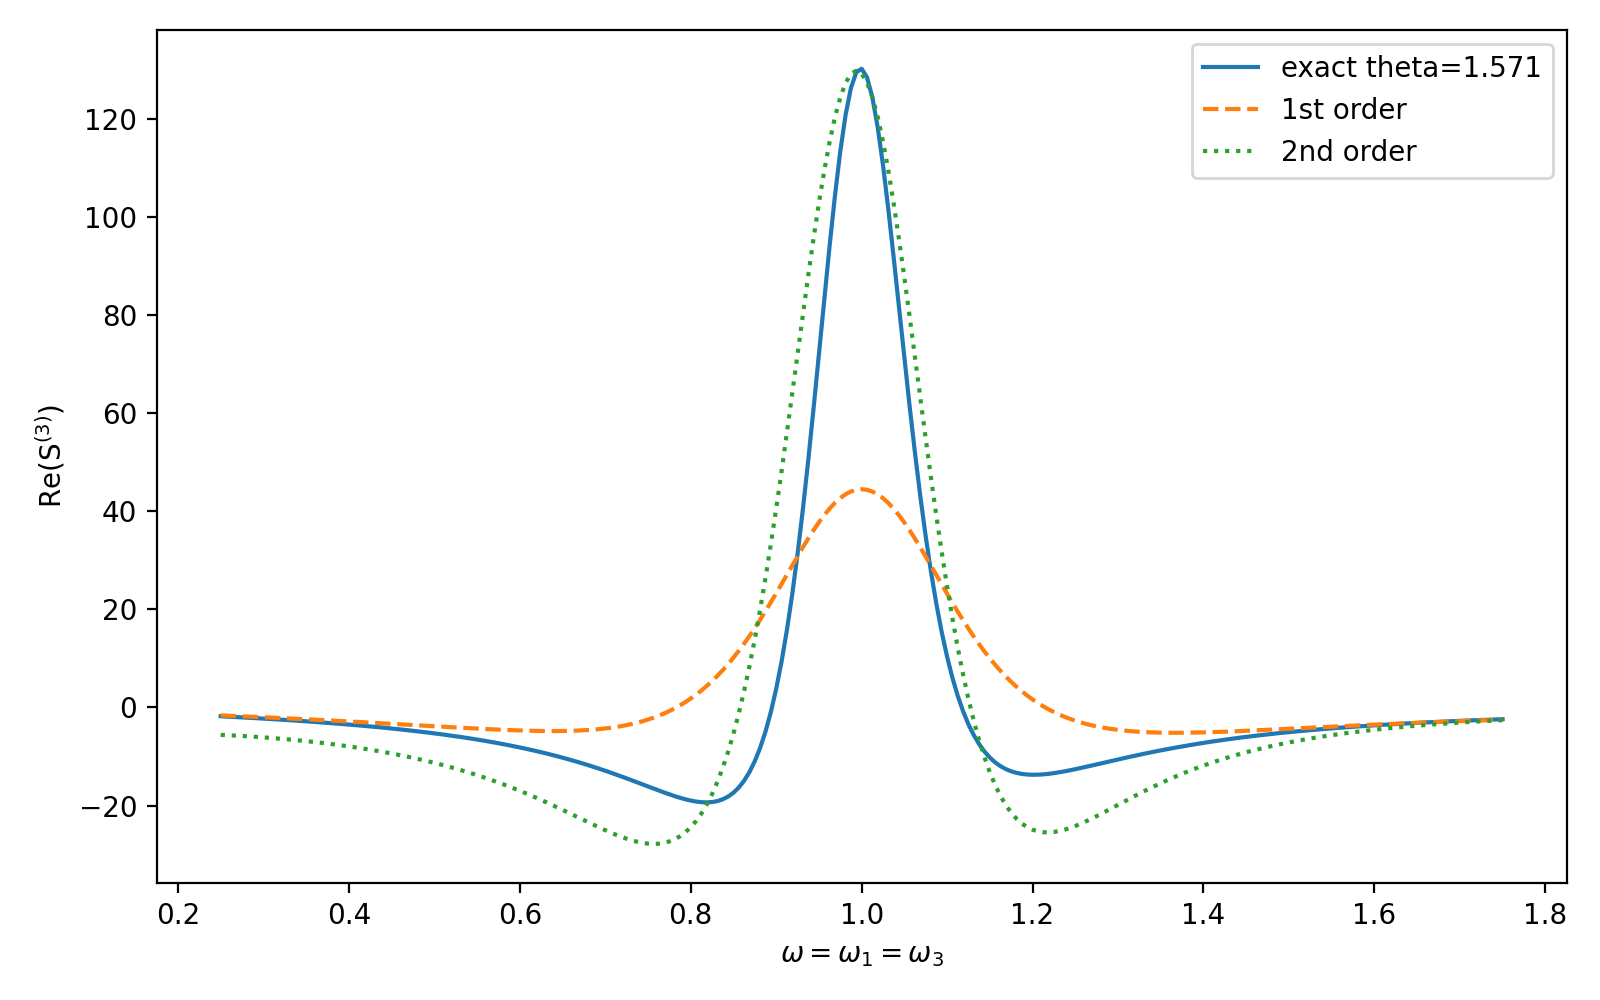
\includegraphics[width=0.48\linewidth]{Figures/duhamel_second_order_real_theta_1p571_2.png}
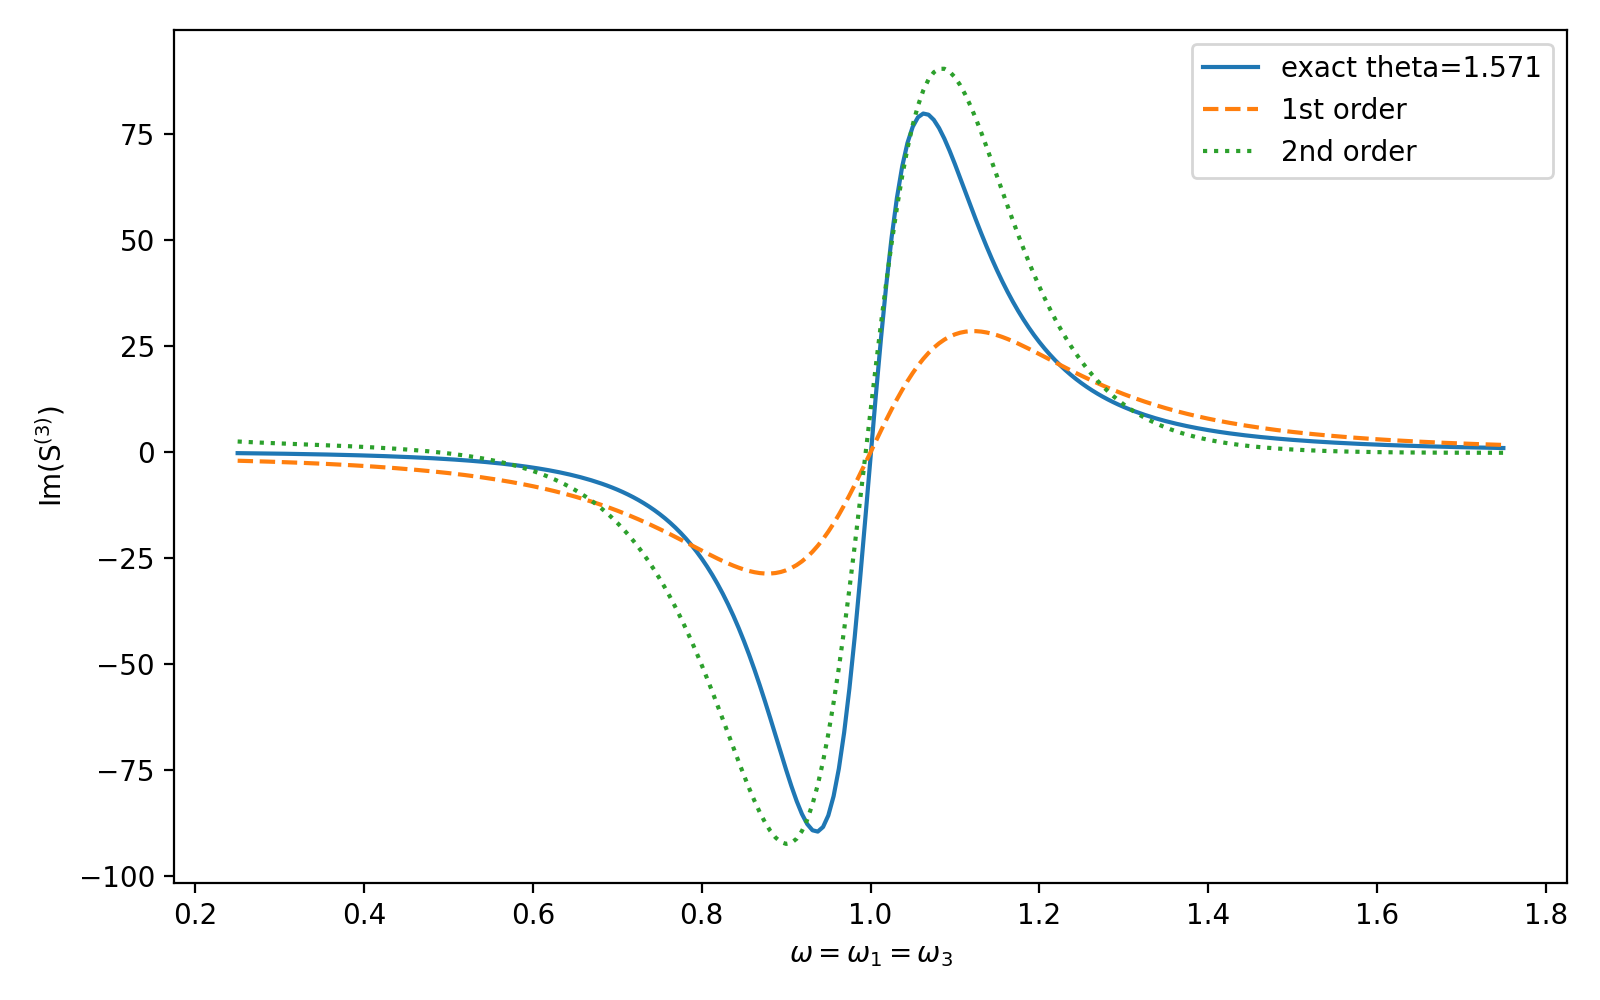
\includegraphics[width=0.48\linewidth]{Figures/duhamel_second_order_imag_theta_1p571_2.png}
\caption{Comparison between exact and reconstructed 
signals at maximal misalignment $\theta = \pi/2$. 
The second-order Duhamel reconstruction reproduces 
the exact response with high fidelity even in this 
strongly deformed regime.}
\label{fig:worst-case}
\end{figure*}


Figure~\ref{fig:worst-case} emphasizes this point by comparing
the exact and reconstructed spectra at
$\theta=\pi/2$, corresponding to maximal observational
deformation. Even in this strongly transported regime the
second-order transport operator accurately reproduces the full
nonlinear response, demonstrating that the dominant geometric
effects are captured by only a small number of transport
coefficients.

\subsection{From Spectral Analysis to Geometric Reconstruction}
The principal conclusion of these calculations is conceptual
rather than numerical. Conventional nonlinear spectroscopy seeks
a microscopic Hamiltonian and dissipative model capable of
reproducing the measured spectrum. Within the present framework,
the objective is instead to reconstruct the local geometry
responsible for the observed response.
The reconstruction proceeds through the hierarchy
\[
P^{(3)}
\Longrightarrow
\theta
\Longrightarrow
T_{ab}
\Longrightarrow
\Gamma_\mu
\Longrightarrow
\mathcal{K}_{\mu\nu},
\]
beginning with experimentally measured spectra and progressing
toward increasingly intrinsic geometric objects. The observable
coordinate determines the local transport operator acting on the
Liouville pathway basis. The transport operator, in turn,
provides direct information about the Liouvillian connection and
its associated curvature.

From this perspective, nonlinear spectroscopy is naturally
reinterpreted as an inverse geometric problem. The measured
spectrum is no longer regarded as the endpoint of the analysis,
but as the observable projection of an underlying response
geometry. Refining the microscopic model therefore becomes
equivalent to refining the local geometry itself, providing a
systematic route toward reconstructing increasingly accurate
Liouvillian manifolds directly from experiment.


